\section*{Supplementary Material}

\subsection*{SI Text}

\subsubsection*{Motivation and Explanation of the Property Violation Game}

At local, regional and global scales, migrations increasingly occur increasingly in uncontrolled ways, with  number of unintended contingencies and challenges for destinations of migration.\\

Likewise, crime and robbery, which aim to destroy or to steal the property of others, relies on fast mobility in neighborhoods, or cities (c.f., gangs in the USA).\\

In the cyberspace, all neighbors are only a few steps away from each others, physically (think of the Internet Protocol (IP) addressing system) or logically through social networks \cite{degree of separation on Facebook}. \\

With unprecedented mobility, invading, destroying or stealing, abusing the assets of people or communities has never been so accessible, leading to concrete consequences for the stability of physical and online societies. According to repeated United Nation reports, mass migration, resulting from wars and climate change, may threaten the stability of long-established societies across the world. Also, for instance, a high crime rate undermines trust among citizen, reduces the enjoyment, and thus often the economic vigor of a city. Similarly, cyber crime and large-scale cyber attacks undermine trust on the cyber space, and thus, its economic potential.\\

Our {\it private-property} model operationalizes the intricate relationship between success-driven migration -- involving an one-sided move perceived as a violation of property by the other side located at a migration distance -- and how it may undermine trust. Trust is characterized by the capability of individuals to engage into cooperation, in a situation where the Nash equilibrium is 0 ( in other words, when both individuals have an individual incentive to defect). The prisoner's dilemma is such a situation where cooperators trust each others.\\

We have tested our model with a variety of parameters, such as population density, migration range, and the probability of property violation, i.e., the probability that an individual may migrate to an occupied site, hence expelling the incumbent individual to another empty location.\\

The rationale for varying the population density stems from the intuition that densely populated areas are more resource intensive (i.e., available resource per individual is more scarce), and thus, in this case, property violation has more negative effects, such as making relocation more difficult for the expelled individual. We indeed found that beyond a given population density (in general when $d > 0.8$), cooperation cannot survive in presence of even the slightest level of property violation.\\

The large span of Moore's migration range, from very local mobility ($M=1$) to levels close to full mobility on the grid (i.e., $M=24$ for a grid of $49\times49$), reflects large inequalities in mobility at local, regional and global scales, also depending on a given environment. For instance, for those having access to the Internet, mobility is unlimited, at least in theory. Also, populations of wealthy social classes can afford traveling nearly all over the world. On the contrary, some individuals have only very limited mobility within a considered environment. The migration range we used shall be viewed as relative to the world under scrutiny: for $M=1$ the individual can only move by $1/24$ of the world size (defined by a grid of size $49\times49$) at each step; for $M=12$, the individual may move within half the size of the world, which is assumed to be uniformly populated. Clusters may form locally but since only one individual can occupy a grid site the density remains overall well distributed, unlike other types of models such as AB models \cite{solomon} in which multiple agents can accumulate on a single site. The migration range applies to all individuals, regardless whether they just migrate to an empty site or if they attempt to expel another player. There is no designated property violator in our model. All individuals may turn property violators based on their payoff opportunity, as well as following their chance to overcome property enforcement.\\

The probability of property violation reflects the limits of property enforcement, whatever the type of enforcement applied, which can be of legal, police and military nature, or as a result of capabilities by individual to protect their own assets. \\


Configurational Analysis of surprises:

\begin{enumerate}
  \item phase transition as a function of $d,M,s$ $\rightarrow$ study actual migration ranges! 
  \item intermediary state with cooperator level steadily $<0.5$
  \item can we ``boot" a world with less than 50\% cooperators with or without property violation? (in particular, show that the game cannot go to a stable state with $c \approx 0.45$ with such initial level?).
  \item high density populations with $s=0$ and $s >0$ 
\end{enumerate}


{\bf In previous research, Helbing and Yu \cite{} have found that We have searched for conter-intuitive situations where property violations would have positive implications for cooperation. So far, we have not found such a result. The intuition for this hypothesis would be that cooperators forced to migrate would create ``unforeseen" situations, which would help spreading cooperation}.

\subsubsection*{Property game step by step: }

\begin{enumerate}
  \item {\bf Player selection: } At each Monte-Carlo Step ($MCS = N \times l \times h$  with $N$ the number of iterations, and $l$ the grid length and $h$ the grid height) a site is selected. If the site is occupied, the {\bf focal player} is selected. Each player is thus expected to be selected $d \times N$ times with $d$ the grid density. 
  
  \item {\bf Success driven migration (exploration) :} With probability $1 - m$, the focal player strategically explores its own migration (Moore) neighborhood $(2M + 1) \times (2M + 1)$ of range $M$, searching for a site with better payoff with her current strategy (either cooperate or defect). To assess for sites with best payoff, the individual plays the prisoner's dilemma with her own strategy and with neighbors for each site within the migration range. For each site assessed, the ``virtual" payoff is computed as the sum of outcomes from playing the prisoner's dilemma with all neighbors.
  
  \item  {\bf Success driven migration (best empty location) :} If among the sites with the highest payoff, some are empty, the player moves to the closest empty site.
  
  \item  {\bf Success driven migration (property violation) :} If there is no empty site among those with highest payoff, the focal player expels the target player with probability $s$. The expelled target player is forced to move to the empty location with highest payoff within her own migration range. The expelled player may find a new empty site with either higher or lower payoff. For both the focal and the target player, in case multiple sites with highest payoff are available, the closest one is automatically selected. If they are at the same distance, one site is randomly chosen among best sites with smallest migration distance.
  
  \item  {\bf Success driven migration (better empty location) :}  If there is no empty site among those with highest payoff and property violation did not occur, the focal player is forced to move to the empty location with higher -- yet not highest -- payoff, with probability $1 - s$.
  
  \item  {\bf Success driven migration (no migration) :} If all empty sites in the migration range have a payoff worse than the incumbent payoff on the focal site, the player does not move.
  
  \item {\bf Random relocation: } With probability $m$, the focal player relocates to a random location either occupied with probability $s$, or to an empty location with probability $1-s$. There is no consideration of random distance in the case of random relocation.
   
 \item {\bf Imitation step :} Whether it has moved or not, the player is allowed to update her strategy (cooperate or defect), by playing the prisoner's dilemma with her neighbors. If one neighbor's strategy leads to a better payoff, the focal player may imitate this strategy with probability $1-r$. With probability $r$, however, her strategy is reset as follows: the player will cooperate with probability $q$ and defect with probability $1-q$. If the (target) player is forced to move after a property violation, she is not allowed to update her strategy (because it is not her turn to play).
\end{enumerate}

\begin{figure}[h!]
\begin{center}
\centerline{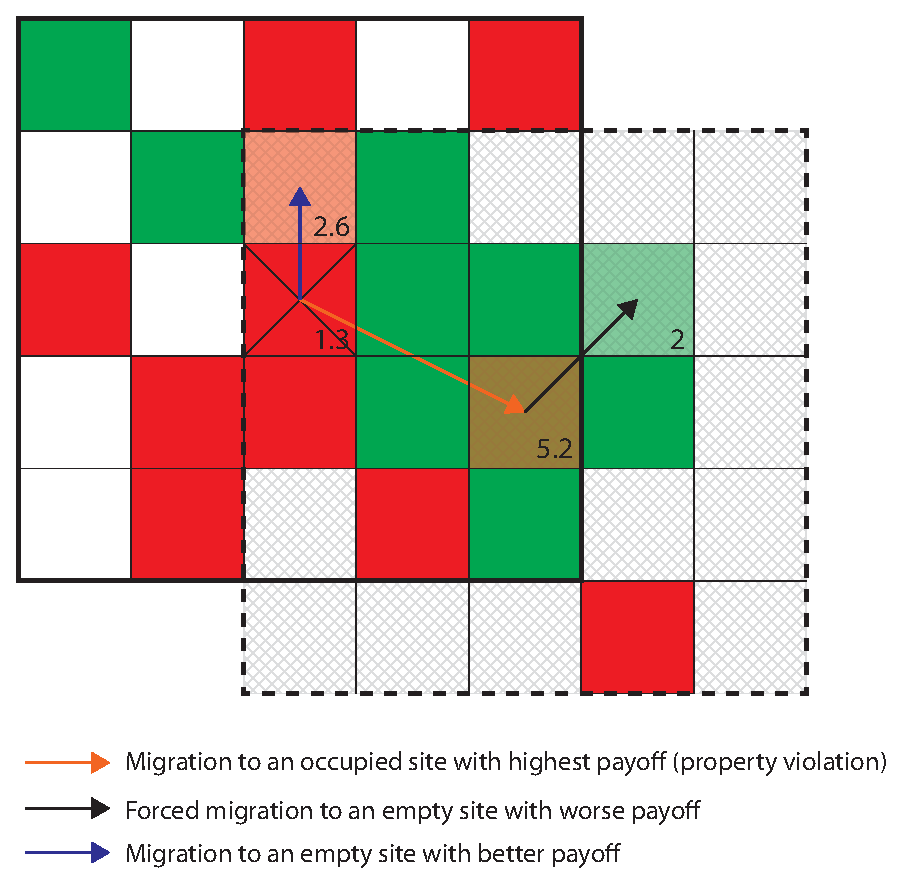
\includegraphics[width=9cm]{../figures/migration_diagram.eps}}
\caption{Migration diagram for focal player on site with payoff $1.3$ (defector on crossed site). The best site in the migration range has highest payoff ($1.3 \times 4 = 5.2$) for a defector, which is the strategy of the focal player. The site with highest payoff is occupied by a cooperative player and may be expelled with probability $s$ (orange arrow). In this case, the player on the target site is forced to move to the nearest empty site with payoff $2$ (black arrow). However, with probability $1-s$, the target player moves to the empty site with payoff ($2.6$) than the payoff at the focal site.}
\label{fig:migration_diagram}
\end{center}
\end{figure}

\subsubsection*{Biological and social coevolution (pasted from Helbing and Yu 2009)}. 
We certainly believe that there
could be a coevolution of social behavior and genetically determined
(��hard-wired��) behavior, as is discussed, for example, by
Gintis and Bowles in their articles on strong reciprocity and
human sociality (2, 3). However, it is still worthwhile to ask how
and why strong reciprocators (who cooperate and punish noncooperators
even if the probability of future interactions is low)
would be ��born�� in sufficient numbers to induce the cooperation
of self-interested agents.
The aforementioned coevolution can be represented by models
assuming group selection. For example, a group containing
a sufficient number of strong reciprocators would have larger
chances of survival in a world characterized by frequent crises
than a group containing no or a few strong reciprocators.
Although the connections between group selection and success-
driven migration are rather limited, one could argue that
individuals with a stronger tendency to cluster have an advantage
over individuals who have a weak tendency to cluster. Moreover,
one could think that there is something like a coevolution
between the strategies individuals choose and their spatial
organization. However, none of this is ��hard-wired�� or genetically
inherited in our model. All individuals in our model are
assumed to be of the same kind, and they do not learn to behave
differently in the course of time (i.e., their behavioral rules or
strategy choices are not history-dependent).

\subsubsection*{Costly punishment (paste from Helbing and Yu 2009)}
 In our model, individuals do not impose a cost
on defectors, but they evade future interactions with them. In
comparison with staying in the neighborhood of defectors, this
reduces the average payoff of defectors and may be considered
as a particular kind of punishment. Therefore, our model may
eventually contribute to a better understanding of emergent
norms, which increase the probability of individuals to show
certain behaviors, thereby making social interactions more predictable
and successful on average.
Note that punishment by evasion is not costly for cooperators
in our model. However, evasion from defectors would be costly,
if we would introduce transaction or relocation costs in our
model. These costs, however, would not be restricted to cooperators.
Whenever defectors move into the neighborhood of
cooperators, they have to pay relocation costs as well. As the
relocation costs of cooperators for evading defectors and the
relocation costs of defectors following cooperators are basically
the same, introducing relocation costs does not change the
conclusions of our study.

$\rightarrow$  Actually the migration range is an implicit cost of relocation: if $M$ is small relocation costs are high and the larger $M$ the less costly migration.

\subsubsection*{Network reciprocity, partner selection, and reputation. (paste from Helbing and Yu 2009} Our model introduces a mechanism for the self-organization of cooperative
clusters (assortment), which differs from the clustering mechanism
observed in spatial games without migration. Assortment
is known to support cooperation, and it is sometimes referred to
by the terms network reciprocity or graph selection. In fact,
moving to cooperative neighborhoods reminds of partner selection
(i.e., the formation of a friendship network with cooperative
individuals, while discontinuing interactions with defecting individuals).
However, forming links with friends requires a reputation
mechanism and, with this, higher cognitive abilities.
In our model, individuals do not need to recognize whether
they have interacted with an individual before and do not
remember what strategy this individual applied. In fact, individuals
do not seek friends, and have little control regarding which
individuals they stay close to and, therefore, which individuals
they interact with. Their neighborhood can, in fact, change
significantly. Moreover, in our model individuals are always
exposed to their neighbors, i.e., they cannot avoid further
interactions with neighbors who defected in the past, if they do
not migrate (but then, they will usually lose contact to their
��friends�� as well). If an individual decides to migrate, the new
neighbors will be interaction partners, no matter whether they
are happy with this or not. Therefore, success-driven migration makes weaker and less
favorable assumptions for cooperation than partner selection.
Although the latter can be very selective and allows the creation
of an individualized interaction network, migration can only
choose among available neighborhoods, which also means that
one may have to accept the presence of defectors, if there are no
better choices.




%\begin{figure}[h]
%\begin{center}
%\centerline{\includegraphics[width=18cm]{../figures/cooperation_M.eps}}
%\caption{Cooperation levels after $N=200$ iterations [i.e., $200 \times 49^2 = 480200$ Monte Carlo Steps (MCS)] for migration Moore's distances $M = \{1,3,5,7,9,11 \}$, as a function of the grid density $d$ and the probability of property violation $s$. At initialization ($i=0$), there is a $50\%$ chance that a player will be a cooperation (resp. defector). The uneven landscapes reflect the statistical fluctuations of simulations. For all $M$, the cooperation exhibits a sharp drop for $d>d^*$  and $s > s^*$ with $(d^*,s^*)$ being a function of $M$. In general, cooperation is only close to 100\% if $d \approx 0$ (or $d = 0$ ?). For $d>0$, cooperation drop at 90\% at best. For high grid density ($d>0.9$), cooperation cannot be sustained even with low property violation ($s > 0$). In presence of property violation ($s>0$), cooperation is best sustained for $s \gg 0$, $M \geqslant 7$ and for grid densities $0.4 < d < 0.6$. These results suggest that mobility $M \gg 0$ is efficient to reduce the effects of property violation, provided that the grid is sufficiently dense (to allow formation of clusters of cooperation) but not overcrowded, hence preventing players expelled from their site to choose a reasonably good site. In the limit $d=1$, property violation reduces to swapping sites, since the only available site in the Moore area is the one left by the property violator. }
%\label{fig:cooperation_M}
%\end{center}
%\end{figure}


%\subsubsection*{Low Populated Worlds ($0 < d \leqslant 0.2$)}


\subsection*{Migration and Property Games in Densely Populated Worlds ($d \geqslant 0.9$)}
\label{SI:d09}

In the success-driven migration game, a fully populated world ($d=1$) is only feasible when property violation exists ($s > 0$), since an individual willing to move must expel another individual. In absence of property violation ($s=0$), the game only involves updating strategies with no migration. When $d=1$ and $s > 0$, we find that cooperators cannot strive and disappear after less than 15 iterations.\\

In the limit of population density $d \rightarrow 1$, success driven migration with property violation $s > 0$ leads to a systematic collapse of cooperation. However, for highly densely populated worlds (e.g., $d = 0.9$), even without property violation ($s = 0$), while cooperators can resist to defectors, they may however {\bf not} be able to invade completely the grid (actually, they may be stuck at an intermediate level, usually $ 0.4 \leqslant c \leqslant 0.6$). Cooperators successfully strive and invade almost completely the grid with some probability, which deserves further scrutiny (see Figure \ref{fig:d1_09_s0_outcomes} for a comparison of games with $d=1$ and with $d=0.9$ with same initial conditions but different outcomes).\\

\begin{figure}[H]
\begin{center}
%\centerline{\includegraphics[width=13cm]{../figures/configuration_d09_s0.eps}}
\caption{Evolution of cooperation for $M=\{1,5,9\}$ for $d=1$ and for $d=0.9$, starting from the same initial conditions of a focal simulation (bold line) for which cooperation could invade more than $90\%$ of the grid.}
\label{fig:d1_09_s0_outcomes}
\end{center}
\end{figure}

Here, we question whether the ability by cooperators to invade the grid, is determined by the initial conditions, or on the contrary, if this capability is the result of a chaotic process, when individuals randomly take their turn for migration and strategy update as the simulation proceed. We performed the simulations ten times for $M=3$ and $M=5$ with random initial conditions, and we repeated 10 times the simulations with each of the 10 initial conditions generated. We then counted the number of simulations that ended with $c > 0.9$, conditioned on random conditions on the one hand, and on fixed initial conditions on the other hand.\\

For $M=3$ (resp. $M=5$), we find that high cooperation achievement $c > 0.9$ results at XX\%  (resp. XX\%) from the initial conditions, and XX\% (resp. XX \%) from the random strategy and migration updates by individuals. The latter contribution may be seen as an instance of a chaotic process.\\

%same initial conditions. We find that the probability that cooperation will manage to invade the grid is 0.XX (see Figure \ref{fig:d09_s0_chaotic}). To account for varying densities, we repeated the test for $d=0.85$ and $d=0.95$ ({\bf [to be done]}.\\


%\begin{figure}[H]
%\begin{center}
%%\centerline{\includegraphics[width=13cm]{../figures/configuration_d09_s0.eps}}
%\caption{Evolution of cooperation for $M=\{3,5,9\}$ and $d=0.9$, starting from the same initial conditions of a focal simulation (bold line) for which cooperation could invade more than $90\%$ of the grid.}
%\label{fig:d09_s0_chaotic}
%\end{center}
%\end{figure}

\begin{figure}[H]
\begin{center}
\centerline{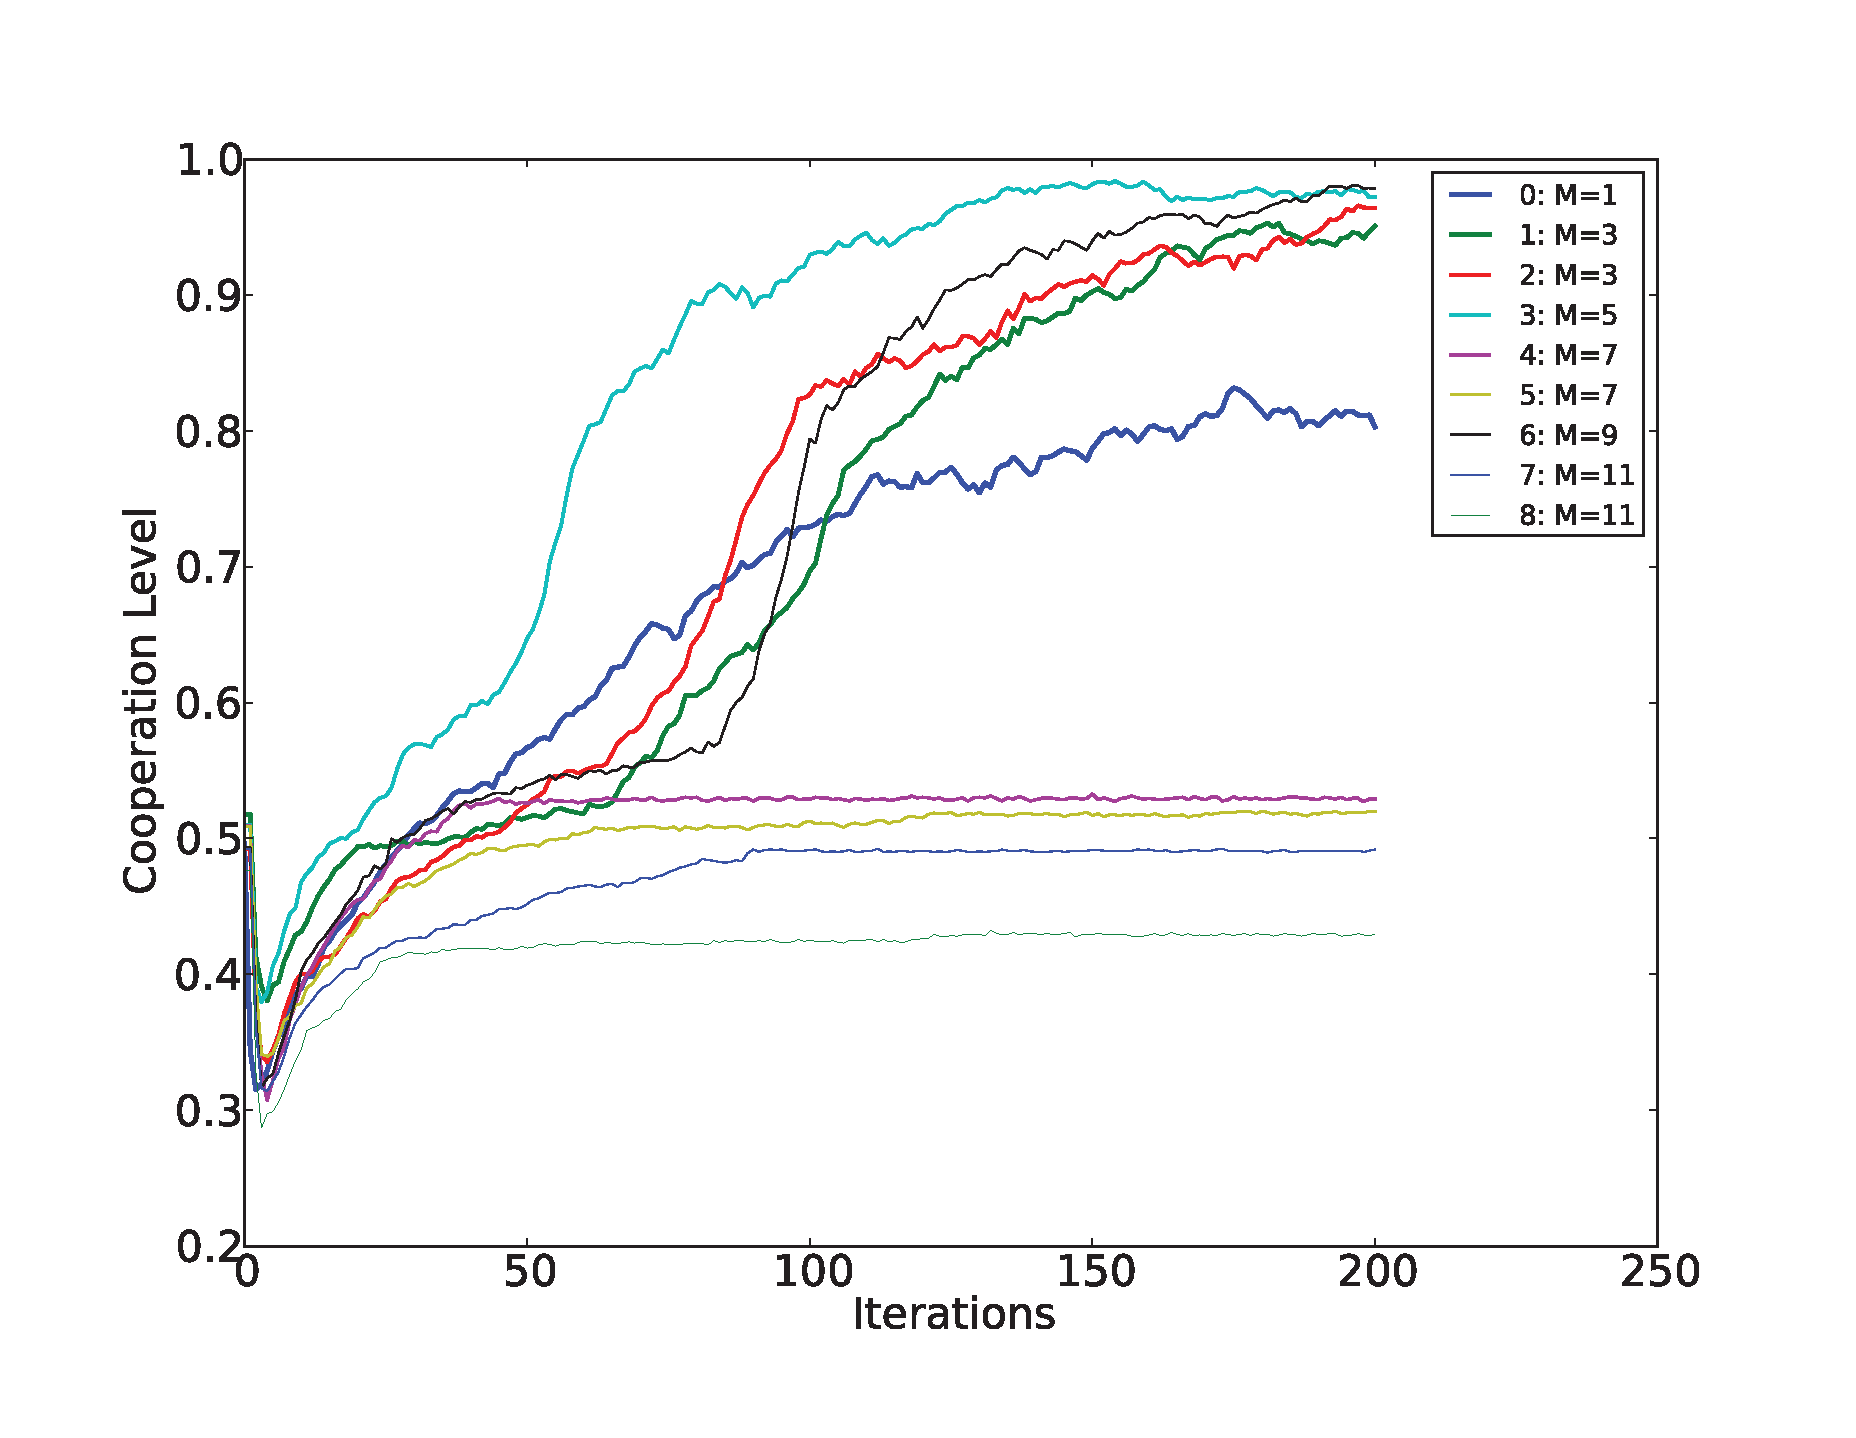
\includegraphics[width=12cm]{../figures/configurations_d09_s0.eps}}
\caption{Evolution of cooperation for $d=0.9$, with $M = \{1,3,5,7,9,11\}$. Cooperation does best for medium migration ranges $M = \{ 3,5\}$. For $M \geqslant 7$, cooperation is stuck between 40\% and 55\%, at the notable exception of $M=9$, which performs as well as $M = \{ 3,5\}$. It looks like that, for all $M$, cooperators counter defector invasion by creating small clusters, which grow up to a saturation where these clusters can survive surrounded by defectors. In some cases $M = \{ 3,5,9\}$, cooperators manage to unlock the situation and further break the belt of defectors. {\bf [The conditions for this to happen remain unclear to me so far, especially that $M=9$ performs like $M = \{ 3,5\}$ rather than like $M = \{ 7,11\}$]}.}
\label{fig:medium_d_migration}
\end{center}
\end{figure}



We shall study in more details the origins of this chaotic behavior, leading either to  $0.4 \leqslant c \leqslant 0.6$ after $t=200$ iterations or to $ c > 0.9$. We inspect how migration patterns in the latter case, influence departure from the former dynamics.\\

\begin{figure}[H]
\begin{center}
\centerline{\includegraphics[width=13cm]{../figures/configuration_d09_s0.eps}}
\caption{Effects of migration in densely populated grids ($d=0.9$). With small migration range $M=1$ (see {\bf B.}), clusters of cooperators form quickly, along with defectors around these clusters. The small migration range does not allow cooperators to jump over defectors. When the migration range is larger $M=5$ (see {\bf C.}), similar clusters of cooperators form at first ($t = 35$), but the larger migration range allows creating connected clusters ($t = 56$), which in turn help overcome most defectors ($t = 200$).}
\label{fig:high_d_migration}
\end{center}
\end{figure}



%\begin{figure}[H]
%\begin{center}
%%\centerline{\includegraphics[width=13cm]{../figures/configuration_d09_s0.eps}}
%\caption{Here a comparison of between a normally continuing simulation, and a sudden drop after $t = 150$ iterations (c.f. time series plots). The hope here is to find a (qualitative) pattern change between these two configurations, which may predict the drop of cooperators.}
%\label{fig:sudden_regime_change}
%\end{center}
%\end{figure}


\clearpage

\subsection*{Migration and Property Games in Medium Populated Worlds ($0.4 \leqslant d \leqslant 6$)}

{\bf [Some text here]}

\begin{figure}[H]
\begin{center}
\centerline{\includegraphics[width=14cm]{../figures/TimeSeriesPhaseTransitions.eps}}
\caption{Evolution of cooperation for average grid density $0.40 \leqslant d < 0.60$ over $N=200$ iterations for migration ranges $M = \{ 1,3,5,7,9,11,13\}$ and for property violation values $s$ close to $s^*(M)$ (migration probability $m=1$). The presented time series illustrate how the property violation phase transition occurs as a function of the migration range. Populations with a small migration range $M=1$ can enhance cooperation after an initial drop. Yet little migration capabilities, make populations very sensitive to property violation: for $s^{*} > 0.05$, defectors win quickly (see {\it A.}). For $M=5$, we observe two scenarios regarding property violation: Either cooperative populations win $s < s^{*} = 0.158$ or on the contrary, they disappear for $s>s^{*}$. It appears that populations, which cannot a sustain a cooperation level higher than $0.5$, almost surely defect  (see {\it B.}). As migration range gets larger ($M = \{7,9\}$), an intermediary state appears, in which populations can sustain clusters of cooperation for some time, while defectors are in majority (see {\it C.} and {\it  D.}). For even larger migration ranges ($M = \{11,13\}$), this intermediary state appears even more clearly (see {\it E.} and {\it  F.}), with cooperative populations in minority ($c \approx 0.45$ for $M=11$ and $c \approx 0.40$ for $M=13$), yet clustered in a world of defectors (see Figure \ref{fig:configurations_t200_M11plus} {\it C} and {\it G}).}
\label{fig:tseries_phase_transition}
\end{center}
\end{figure}


%\begin{figure}[H]
%\begin{center}
%\centerline{\includegraphics[width=13cm]{../figures/configuration_d05_s0.eps}}
%\caption{}
%\label{fig:medium_d_migration}
%\end{center}
%\end{figure}


\begin{figure}[H]
\begin{center}
\centerline{\includegraphics[width=13cm]{../figures/configuration_d05_s0.eps}}
\caption{}
\label{fig:medium_d_migration}
\end{center}
\end{figure}

